\documentclass[12pt]{article}
\usepackage{latexsym,amssymb,amsmath} % for \Box, \mathbb, split, etc.
% \usepackage[]{showkeys} % shows label names
\usepackage{cite} % sorts citation numbers appropriately
\usepackage{path}
\usepackage{url}
\usepackage{verbatim}
\usepackage[pdftex]{graphicx}

% horizontal margins: 1.0 + 6.5 + 1.0 = 8.5
\setlength{\oddsidemargin}{0.0in}
\setlength{\textwidth}{6.5in}
% vertical margins: 1.0 + 9.0 + 1.0 = 11.0
\setlength{\topmargin}{0.0in}
\setlength{\headheight}{12pt}
\setlength{\headsep}{13pt}
\setlength{\textheight}{625pt}
\setlength{\footskip}{24pt}

\renewcommand{\textfraction}{0.10}
\renewcommand{\topfraction}{0.85}
\renewcommand{\bottomfraction}{0.85}
\renewcommand{\floatpagefraction}{0.90}

\usepackage{accents}
\newcommand{\ubar}[1]{\underaccent{\bar}{#1}}
\makeatletter
\setlength{\arraycolsep}{2\p@} % make spaces around "=" in eqnarray smaller
\makeatother
\usepackage{stackengine}
% change equation, table, figure numbers to be counted inside a section:
\numberwithin{equation}{section}
\numberwithin{table}{section}
\numberwithin{figure}{section}

% begin of personal macros
\newcommand{\half}{{\textstyle \frac{1}{2}}}
\newcommand{\eps}{\varepsilon}
\newcommand{\myth}{\vartheta}
\newcommand{\myphi}{\varphi}

\newcommand{\IN}{\mathbb{N}}
\newcommand{\IZ}{\mathbb{Z}}
\newcommand{\IQ}{\mathbb{Q}}
\newcommand{\IR}{\mathbb{R}}
\newcommand{\IC}{\mathbb{C}}
\newcommand{\Real}[1]{\mathrm{Re}\left({#1}\right)}
\newcommand{\Imag}[1]{\mathrm{Im}\left({#1}\right)}
\DeclareRobustCommand{\brkbinom}{\genfrac[]{0pt}{}}
\newcommand{\norm}[2]{\|{#1}\|_{{}_{#2}}}
\newcommand{\abs}[1]{\left|{#1}\right|}
\newcommand{\ip}[2]{\left\langle {#1}, {#2} \right\rangle}
\newcommand{\der}[2]{\frac{\partial {#1}}{\partial {#2}}}
\newcommand{\dder}[2]{\frac{\partial^2 {#1}}{\partial {#2}^2}}
\usepackage{enumitem}
\newcommand{\nn}{\mathbf{n}}
\newcommand{\xx}{\mathbf{x}}
\newcommand{\uu}{\mathbf{u}}
\usepackage{tikz}
\usetikzlibrary{arrows}
\usetikzlibrary{positioning}
\usepackage{titlesec}
\newcommand{\junk}[1]{{}}
\usepackage{sectsty}
\usepackage{xcolor}
\newcommand*{\bfrac}[2]{\genfrac{}{}{0pt}{}{#1}{#2}}
\newcommand\myatop[2]{\left[{{#1}\atop#2}\right]} % "wrapper macro"
\usepackage{array}
\usepackage{multirow}
\usepackage{amsmath}
\DeclareMathOperator*{\argmax}{arg\,max}
\DeclareMathOperator*{\argmin}{arg\,min}
\makeatletter
\renewcommand*\env@matrix[1][\arraystretch]{%
	\edef\arraystretch{#1}%
	\hskip -\arraycolsep
	\let\@ifnextchar\new@ifnextchar
	\array{*\c@MaxMatrixCols c}}
\makeatother

\makeatletter
\renewcommand*\env@matrix[1][*\c@MaxMatrixCols c]{%
	\hskip -\arraycolsep
	\let\@ifnextchar\new@ifnextchar
	\array{#1}}
\makeatother

\definecolor{darkblue}{rgb}{0,0,0.4}
\usepackage[colorlinks = true,
linkcolor = darkblue,
urlcolor  = darkblue,
citecolor = darkblue,
anchorcolor = darkblue]{hyperref}
% set two lengths for the includegraphics commands used to import the plots:
\newlength{\fwtwo} \setlength{\fwtwo}{0.45\textwidth}
% end of personal macros

\begin{document}
\DeclareGraphicsExtensions{.jpg}

\begin{center}
\textsc{\Large Statistical Pattern Recognition} \\[2pt]
	\textsc{\large Assignment 4}\\
	\vspace{0.5cm}
  Ali Gholami \\[6pt]
  Department of Computer Engineering \& Information Technology\\
  Amirkabir University of Technology  \\[6pt]
  \def\UrlFont{\em}
  \url{https://aligholamee.github.io}\\
    \href{mailto:aligholami7596@gmail.com}{\textit{aligholami7596@gmail.com}}
\end{center}

\begin{abstract}
In statistics, kernel density estimation (KDE) is a non-parametric way to estimate the probability density function of a random variable. Kernel density estimation is a fundamental data smoothing problem where inferences about the population are made, based on a finite data sample. In some fields such as signal processing and econometrics it is also termed the Parzen-Rosenblatt window method, after Emanuel Parzen and Murray Rosenblatt, who are usually credited with independently creating it in its current form. (Summarization from Wikipedia)
\end{abstract}

\subparagraph{Keywords.} \textit{KNN Classifier, Kernel Density Estimation.}

\section{Parzen Windows with Gaussian Kernels}
Generate 100 random points from each of the following two distributions: $N(20, 5)$ and $N(35, 5)$. Write a program that employs Parzen window technique with a Gaussian kernel to estimate density using all 200 points. Note that this density conforms to a single bimodal distribution (a Gaussian Mixture Model).

\begin{enumerate}[label=(\alph*)]
	\item Plot the estimated density function for each of the following window widths: h = 0.01, 0.1, 1, 10. [Note: You can estimate the density at discrete values of x in the [0, 55] interval with a step-size of 1.]
	
	\item Repeat the above after generating (i) 500 training points from each of the two distributions, (ii) 1,000 training points from each of the two distributions; and (iii) 2,000 training points from each of the two distribution.
	
	\item Discuss how the estimated density changes as a function of the window width and the number of training points.
\end{enumerate}

\subsection*{Solution}
\begin{enumerate}[label=(\alph*)]
	\item The following items are generated by the Python file under the directory: \textit{src/1}.
	
	Suppose $h = 0.01$. The results is given in figure 1.1.
		\begin{figure}[!h]\centering
		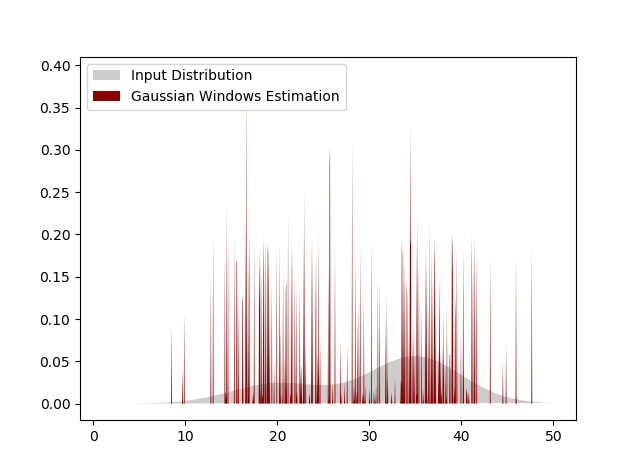
\includegraphics[width=0.6\textwidth]{1_a_1.PNG}
		\caption{Density Estimation with Gaussian Kernels: $h = 0.01$.}
		\label{pl1}
	\end{figure}

	Suppose $h = 0.1$. Plotted densities are given in figure 1.2.
			\begin{figure}[!h]\centering
		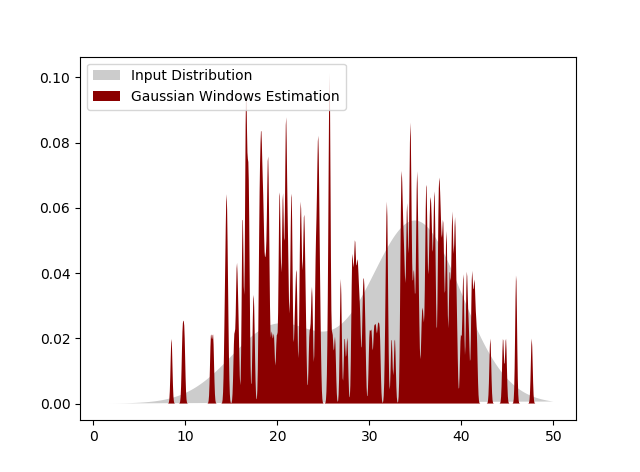
\includegraphics[width=0.6\textwidth]{1_a_2.PNG}
		\caption{Density Estimation with Gaussian Kernels: $h = 0.1$.}
		\label{pl1}
	\end{figure}
	
	Suppose $h = 1$. The results is given in figure 1.3.
	\begin{figure}[!h]\centering
		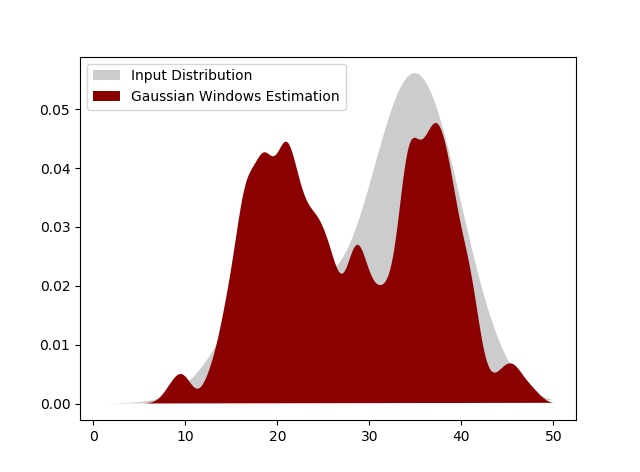
\includegraphics[width=0.6\textwidth]{1_a_3.PNG}
		\caption{Density Estimation with Gaussian Kernels: $h = 1$.}
		\label{pl1}
	\end{figure}

	Suppose $h = 10$. The results is given in figure 1.4.
	\begin{figure}[!h]\centering
		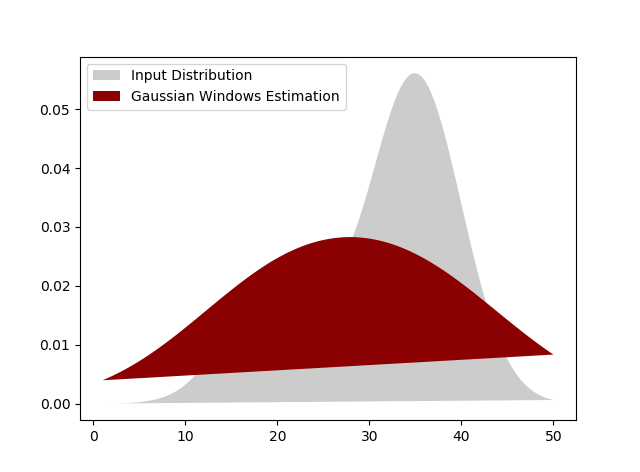
\includegraphics[width=0.6\textwidth]{1_a_4.PNG}
		\caption{Density Estimation with Gaussian Kernels: $h = 10$.}
		\label{pl1}
	\end{figure}

\item Here is the repeated procedure for 500 number of points for $h = 1$. Results is given in figure 1.5. It is obvious that the accuracy of estimation is higher in this case.
	\begin{figure}[!h]\centering
	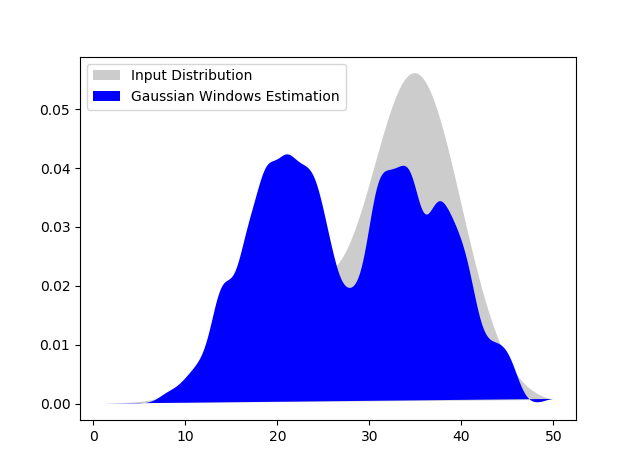
\includegraphics[width=0.6\textwidth]{1_b_1.PNG}
	\caption{Density Estimation with Gaussian Kernels: $h = 1$, $500$ Samples.}
	\label{pl1}
\end{figure}

Results for $1000$ number of samples is provided in figure 1.6.
	\begin{figure}[!h]\centering
	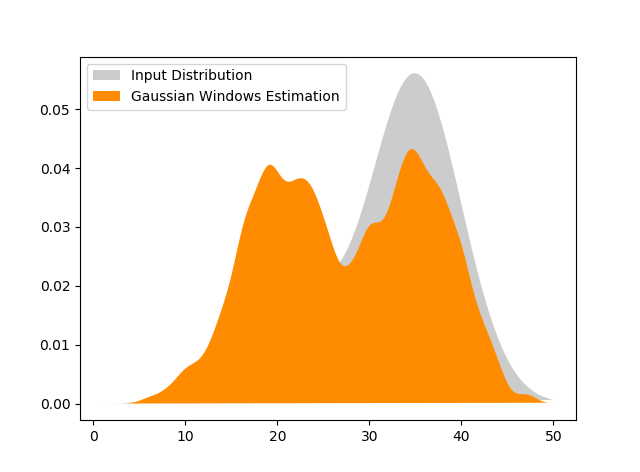
\includegraphics[width=0.6\textwidth]{1_b_2.PNG}
	\caption{Density Estimation with Gaussian Kernels: $h = 1$, $1000$ Samples.}
	\label{pl1}
\end{figure}

Final results for $2000$ samples is provided in figure 1.7.
	\begin{figure}[!h]\centering
	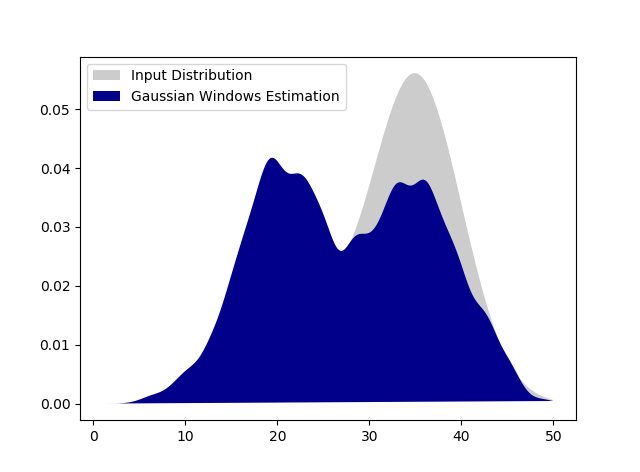
\includegraphics[width=0.6\textwidth]{1_b_3.PNG}
	\caption{Density Estimation with Gaussian Kernels: $h = 1$, $2000$ Samples.}
	\label{pl1}
\end{figure}

\item For any choice of kernel, the bandwidth h is a smoothing parameter, and controls how smooth the fit is by controlling the size of the neighbourhood around the reference, x0.

If h is large, we consider a large neighborhood, and vice versa.

In the Gaussian kernel case, varying h has the same effect as varying the variance of a Gaussian. Small h leads to a thinner, more peaked Gaussian, whereas larger h leads to a fatter Gaussian, in the extreme case, closer and closer to a flat line.

On the other hand, when the number of samples increase, the accuracy of the estimation goes high. This simply means that the bias of the estimation goes down.
\end{enumerate}

\section{Kernel Density Estimation \& KNN Estimation}
Given dataset $ X = 2, 3, 4, 4, 4, 5, 5, 10, 11, 11, 11, 12, 14, 16 $ use Parzen windows to estimate density $p(x)$ at $x = 5$ and $x = 12$; assuming $h = 4$ in the following conditions.
\begin{enumerate}[label=(\alph*)]
	\item If you use standard kernel function
	\[ K(u) =
	\begin{cases}
	1      & \quad |u| \leq \frac{1}{2}\\
	0  & \quad o.w.
	\end{cases}
	\]


	\item If you use Gaussian Kernel, $N(0, 1)$.
	
	\item For the same dataset and the same sample points, i.e. $x = 5$ and $x = 12$, estimate the density using KNN approach. Take $ K = 5$ in your estimations.

\end{enumerate}

\subsection*{Solution}
\begin{enumerate}[label=(\alph*)]
	\item We'll use (1.1) to estimate the density using different kernels.
	\begin{equation}
	\hat{p}_{(x)} = \frac{1}{n*h^d} \sum_{i = 1}^{k}\Phi(\frac{x - x_i}{h})
	\end{equation}
	In this case, we'll compute the distance of each of the given points from our dataset. For every distance less than 2 we'll consider the effect of that point in our estimation.
	$$
		x = 5\ \ \ \rightarrow\ \ \ \hat{p}_{(x)} = \frac{1}{14 * 4} * (6) = \frac{3}{28} = 0.107
	$$
	Doing the same for the point $x = 12$ and we'll have the following results:
	$$
		x = 12\ \ \ \rightarrow\ \ \ \hat{p}_{(x)} = \frac{1}{14 * 4} * (6) = \frac{3}{28} = 0.107
	$$
	
	\item In this case, the value of items in the $\sum$ are no longer 1. They will have different outputs, specially on the center of the curve. This can lead to an smoother and more realistic estimation of the density. The Gaussian Kernel equation is given in (1.2).
	\begin{equation}
		\phi(u) = \frac{1}{\sqrt{2\pi}}\exp(\frac{-u^2}{2})
	\end{equation}
	
	$$
		x = 5\ \ \ \rightarrow\ \ \ \hat{p}_{(x)} = \frac{1}{14 * 4} * \frac{1}{\sqrt{2\pi}} (\exp(-2) + 3\exp(\frac{-1}{2}) + 2)) = 0.028
	$$
	
	$$
		x = 12\ \ \ \rightarrow\ \ \ \hat{p}_{(x)} = \frac{1}{14 * 4} * \frac{1}{\sqrt{2\pi}} (2\exp(-2) + 3\exp(\frac{-1}{2}) + 1)) = 0.021
	$$
	
	\item In this case, we have to consider the window size as a dynamic variable. In case $h = 2$ then $x = 4$, $x = 4$, $x = 4$ and $x = 5$ will be in our window of estimation as well as the centered point $x = 5$ (K = 5). To estimate the density we'll have the following equation:
	$$
		x = 5\ \ \ \rightarrow\ \ \ \hat{p}_{(x)} = \frac{1}{14 * 2} * (5) = 0.178
	$$
	Note that we have considered the kernel to be the same as part a. In the second case, choosing the $h = 2$ yields 5 points.
	$$
	x = 12\ \ \ \rightarrow\ \ \ \hat{p}_{(x)} = \frac{1}{14 * 2} * (5) = 0.178
	$$
\end{enumerate}

\section{Parzen Windows \& KNN Estimation}
Consider the following training set drawn from an unknown density $f(x)$:
$$
	X = \{ 0.01, 0.12, 0.19, 0.32, 0.41, 0.48\}
$$
\begin{enumerate}[label=(\alph*)]
		
	\item	Let $\phi(x) = N(0, 1)$. Find and sketch the Parzen Windows estimate for the values of $h_n$ of $0.1$ and $1.0$.
	\begin{equation}
	\hat{f_n}_{(x)} = \frac{1}{n*h_n} \sum_{i = 1}^{k}\Phi(\frac{x - x_i}{h_n})
	\end{equation}
	
	
	\item Find and sketch the 3-nearest neighbor estimate of $f(x)$.
\end{enumerate}

\section*{Solution}

\begin{enumerate}[label=(\alph*)]
	\item For each point in our dataset, we'll center the Gaussian Kernel and add the values of these kernels. Here are the computations in case that $h_n = 0.1$.
	$$
	\hat{f_n}_{(x = 0.01)} = \frac{1}{6*0.1} *1  = 1.66 \ \ \ \ \hat{f_n}_{(x = 0.12)} = \frac{1}{6*0.1} * 1= 1.66
	$$

	$$
	\hat{f_n}_{(x = 0.19)} = \frac{1}{6*0.1} * 1 = 1.66 \ \ \ \ \hat{f_n}_{(x = 0.32)} = \frac{1}{6*0.1} * 1 = 1.66
	$$
	$$
	\hat{f_n}_{(x = 0.41)} = \frac{1}{6*0.1} * 1 = 1.66\ \ \ \ 	\hat{f_n}_{(x = 0.48)} = \frac{1}{6*0.1} * 1 = 1.66
	$$
	As denoted above, estimation will give 0 for all of the points in the dataset with $h_n = 0.1$. We can understand that, the window size has been chosen too small that no point is being considered by the estimator. Note that the $h = 0.1$ will be divided by 2 (Being symmetric) and the neighborhood of each given point in the dataset is checked with a diameter of $0.05$. In this case, non of the windows contained other points. Since we have considered the point itself having an effect on the density (As in previous problem), we'll consider them here also.
	In this case, the density estimation plot is given in the figure 3.1.
	\begin{figure}[!h]\centering
	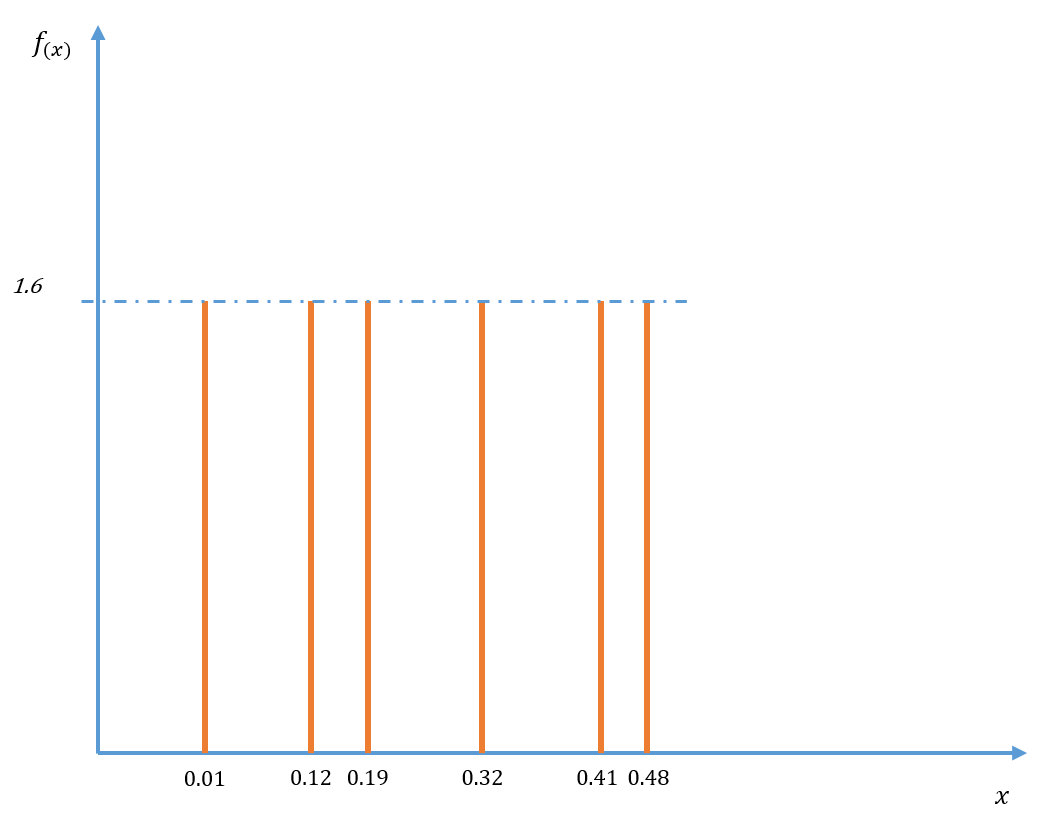
\includegraphics[width=0.6\textwidth]{2_a_1.PNG}
	\caption{Kernel Estimation of f(x) with $h_n = 0.1$.}
	\label{pl1}
	\end{figure}
	
	In the second case, the window size is $h_n = 1.0$. For each point in the dataset, if we put a window of size 1.0 on that point, all other points are included in the window. We can understand that in this case, the window size is too large. $f(x)$ estimation is given below.
	
	$$
		\hat{f_n}_{(x =0.01)} = \frac{1}{6*0.1} * (exp(0) + exp(\frac{-0.0121}{2}) +
		 exp(\frac{-0.0324}{2}) + exp(\frac{-0.0961}{2}) + 
	$$
	$$
	exp(\frac{-0.16}{2}) + exp(\frac{-0.2209}{2}) = 0.95
	$$
	\newpage
	This procedure is same for all of the given points in the dataset. In the case of window size of 0.1, the estimation results is given in the figure 3.2.
	\begin{figure}[!h]\centering
		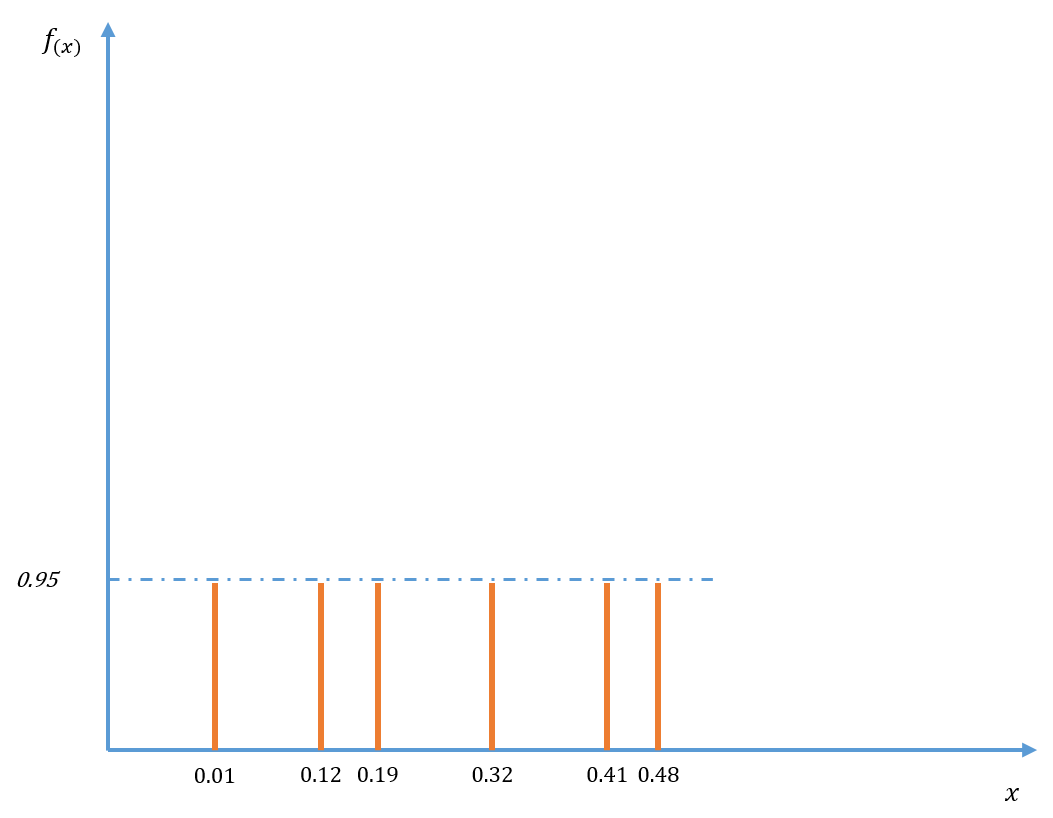
\includegraphics[width=0.6\textwidth]{2_a_2.PNG}
		\caption{Kernel Estimation of f(x) with $h_n = 1$.}
		\label{pl1}
	\end{figure}


	\item In this section, we'll start from $h_n = 0$. We'll gradually increase the value of $h_n$ until the window includes 3 samples. Starting from $x = 0.01$, suppose $h = 0.2$. Only 2 samples are included in the window. Increasing the window size to $h = 0.4$ will properly include 3 samples which is denoted by $ k = 3$. Thus, for the first sample, the proper window size is $h_n = 0.4$. The estimated value will be:
	$$
		\hat{f_n}_{(x = 0.01)} = \frac{1}{6*0.4} * (exp(0) + exp(\frac{-0.0121}{2}) + exp(\frac{-0.0324}{2})) = \frac{2.71}{2.4} = 1.12
	$$

	$$
	\hat{f_n}_{(x = 0.12)} = \frac{1}{6*0.22} * (exp(\frac{-0.0121}{2})+ exp(0) + exp(\frac{-0.0049}{2})) = \frac{2.99}{1.32} = 1.24
	$$
	Continuing this procedure for all of the points in the dataset yields the figure 3.3.
	$$
		\hat{f_n}_{(x = 0.19)} = \frac{2.97}{1.56} = 1.9
	$$
	$$
		\hat{f_n}_{(x = 0.32)} = \frac{2.97}{1.56} = 1.9
	$$
	
	$$
		\hat{f_n}_{(x = 0.41)} = \frac{2.98}{1.08} = 2.75
	$$
	
	$$
		\hat{f_n}_{(x = 0.48)} = \frac{2.96}{1.92} = 1.54
	$$
	\begin{figure}[!h]\centering
		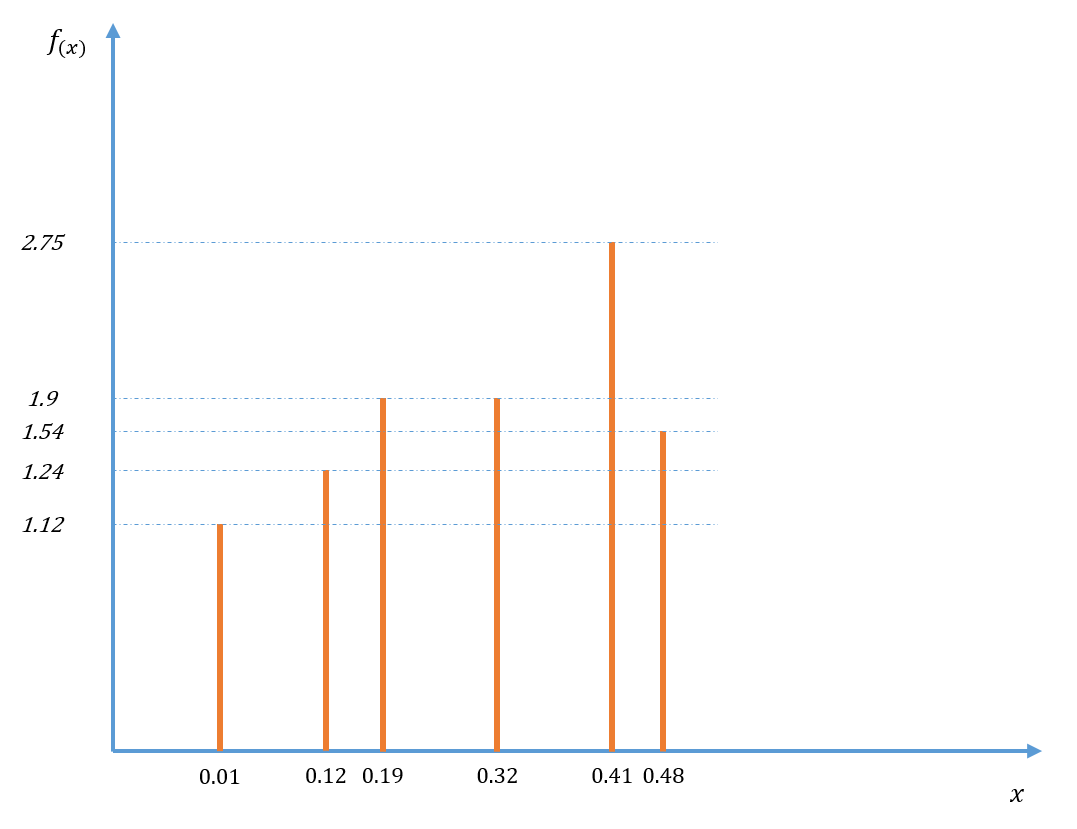
\includegraphics[width=0.6\textwidth]{2_b.PNG}
		\caption{Kernel Estimation of f(x) with KNN Estimator with $K = 3$.}
		\label{pl1}
	\end{figure}
\end{enumerate}

\section{KNN Decision Boundary \& Voronoi Cells}
In the following questions you will consider a K-Nearest Neighbor classifier using Euclidean distance metric on a binary classification task.

\begin{enumerate}[label=(\alph*)]
	\item Sketch the 1-Nearest Neighbor decision boundary for this dataset.
	\begin{figure}[!h]\centering
		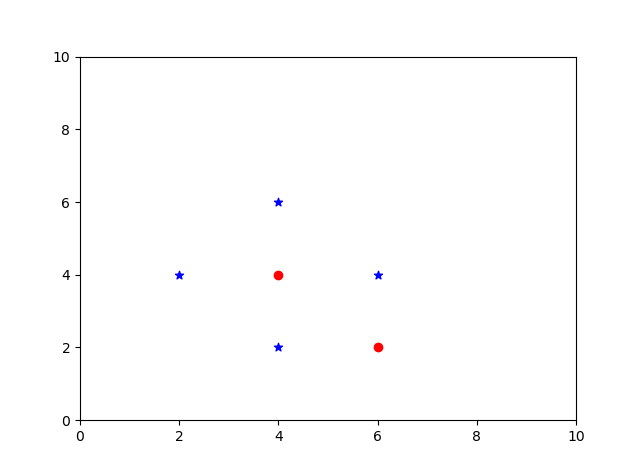
\includegraphics[width=0.7\textwidth]{3_1.png}
		\label{pl1}
	\end{figure}


	\item How would the point (8, 1) be classified using 1-NN?
\end{enumerate}


\subsection*{Solution}
\begin{enumerate}[label=(\alph*)]
	\item The decision boundary for 1-NN is given in figure 4.1.
	
	\begin{figure}[!h]\centering
		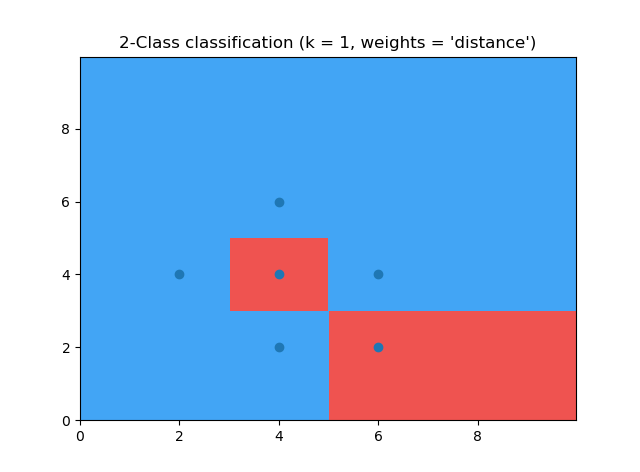
\includegraphics[width=0.7\textwidth]{3_2.png}
		\caption{1-NN Decision Boundaries \& Voronoi Cells.}
		\label{pl1}
	\end{figure}

	\item It will be classified as red, as the regions are given in figure 4.1.
\end{enumerate}

\section{KNN Decision Boundary \& KNN Error Rate}
Consider a K-Nearest Neighbor classifier using Euclidean distance metric on a binary classification task.
	\begin{figure}[!h]\centering
	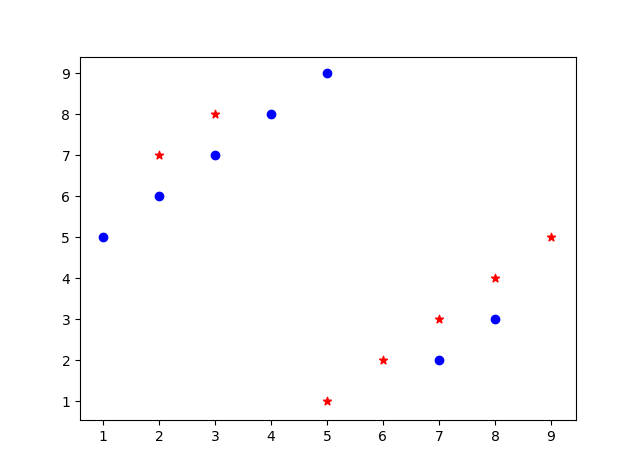
\includegraphics[width=0.7\textwidth]{4.png}
	\label{pl1}
\end{figure}
\begin{enumerate}[label=(\alph*)]
	\item In the figure, sketch the 1-Nearest Neighbor decision boundary for this dataset.
	\item If you try to classify the entire training dataset using a K-NN classifier, what value of K will minimize the error for this dataset?
	\item What happens if you use a very large K on this dataset? Why might too small values of K also be bad?
\end{enumerate}
\newpage
\subsection*{Solution}
\begin{enumerate}[label=(\alph*)]
	\item 	Here is the results plotted using Matplotlib in Python.
	\begin{figure}[!h]\centering
		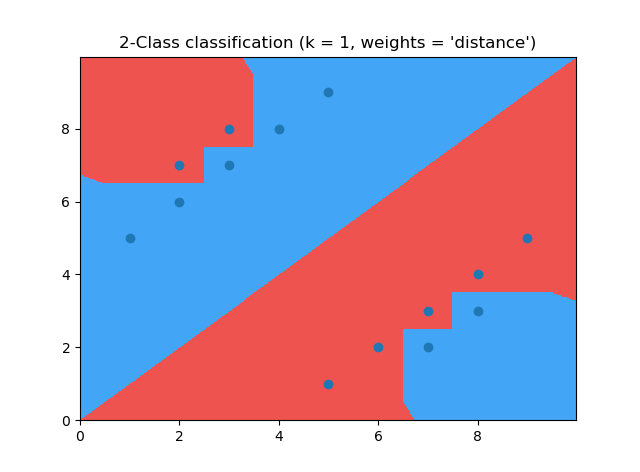
\includegraphics[width=0.7\textwidth]{4_2.png}
		\caption{1-NN Decision Boundaries \& Voronoi Cells.}
		\label{pl1}
	\end{figure}

	\item K can be found using experiments. The code is provided in the \textit{src} folder.
	
	\item Using large K's yields in a smaller degree of freedom. Thus, it prevents the classifier from overfitting. Too small values for K result in a higher degree of freedom. This results in an overfitted model.
\end{enumerate}
\end{document} 

